\chapter{The Milky Way Galaxy}\label{chap:milkyway}
\section{Components}\label{sec:components}
\begin{figure}[t]
    \centering
    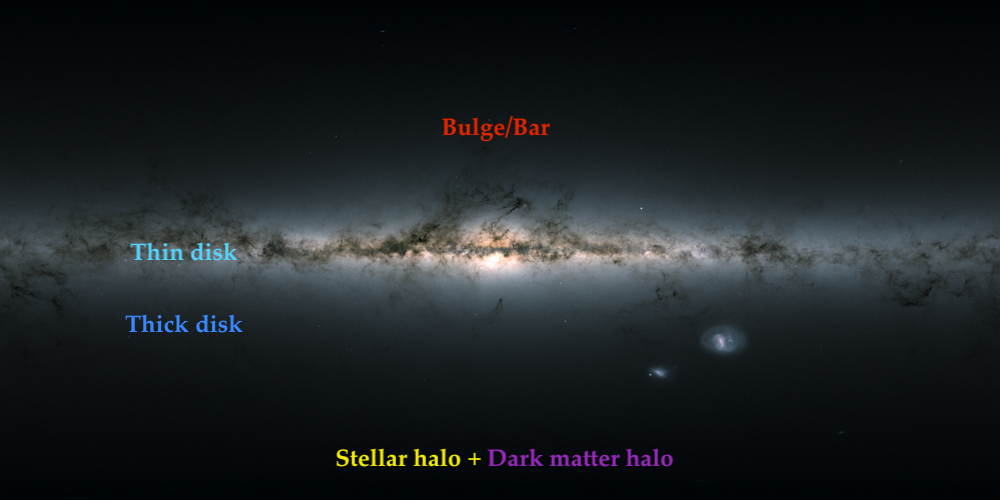
\includegraphics[width=1\textwidth]{images/gaiasky.png}
    \caption{All-sky view of the Milky Way Galaxy from Gaia based on measurements of nearly 1.7 billion stars. We mark the location of different components of the Galaxy with different colors. {\color{red} Get permission to adjust/use image contact \textit{spaceinimages@esa.int}}.} % Fig. 1.1
    \label{fig:gaiasky}
\end{figure}
All throughout history mankind has sought to understand the night sky and its many features such as stars, clumps, planets or `wanderers'. But no feature is as large and noticeable as the great spray of stars that make up the Milky Way Galaxy, named so for the milk from Hera's breast in Greek mythology \citep{leeming:98}. The suggestion that this milky band of stars was a rotating body, of which we the observers are inside, came not until \cite{wright:1750}. Since then our understanding of our home Galaxy has increased tremendously and we can present stunningly detailed views of it like the map shown in Fig. \ref{fig:gaiasky}. This map is made possible thanks to measurements from Gaia's second data release (\citealt{dr2},  herafter DR2). As the figure shows the Milky Way is composed of several different components with stars differing in spatial distribution, kinematics, chemistry, and age. Since the three papers together touch upon almost every component mentioned in Fig. \ref{fig:gaiasky} we will briefly provide a description of each one.

\subsection{Thin disk}
The thin disk is what visually makes up the Milky Way and since it is where the Sun is located it is the the most well-studied of the stellar components. The thin disk is also the site of ongoing star formation which recent estimates place as high as $\approx 3.3\ \mathrm{M_\odot yr}^{-1}$ \citep{zari:22}. As the name suggests it is relatively thin with a scale length of $R_\mathrm{t} \approx 2.6$ kpc, scale height of $z_\mathrm{t} \approx 300$ pc, and with a mass $M_\mathrm{t} \approx 3.5\times 10^10$ M$_\odot$ \citep{bland-hawthorn:16}. The thin disk stars are generally younger and has an abundance of $\alpha$-elements similar to the sun. We measure the abundances as:
\begin{equation}
    [\alpha/\mathrm{Fe}] = \log_{10}\left(\frac{N_\alpha}{N_\mathrm{Fe}}\right)_\mathrm{star} - \log_{10}\left(\frac{N_\alpha}{N_\mathrm{Fe}}\right)_\odot,
\end{equation}
where $N$ is the number of atoms per unit of volume.

\subsection{Thick disk}
The second disk of the Galaxy fulfills its name with a scale height of $z_\mathrm{T}\approx 900$ pc, scale length $R_\mathrm{T} \approx 2$ kpc, and mass $M_\mathrm{T} \approx 6$ M$_\odot$ \citep{bland-hawthorn:16}. It's stars are older \citep{martig:16} and kinematically hotter, since age and velocity dispersion are correlated (\citealt{martig:14,aumer:16}). In metallicity space, thick disc stars occupy regions of higher [$\alpha$/Fe] and have been tentatively linked to the high-$\alpha$ sequence \citep{katz:21}. How the thick and thin discs formed is still a debated topic, particularly so the former as explained in \cite{helmi:20} who also shows that the formation may be related to the evolution of the stellar halo through mergers with nearby galaxies. 

\subsection{Stellar halo}
The most extended component is the stellar halo which contains $1.3^{+0.3}_{-0.2} \times 10^9$ M$_\odot$ within $2 < r < 70$ kpc \citep{mackereth:20} and is host to the oldest and most metal-poor stars in the Galaxy \citep{dacosta:19, horta:22}. The orbits of halo stars is more spherical than the disks and so can be told apart locally by their kinematics. Relative to the discs, the halo stars will appear to move with a speed of 200 km s$^{-1}$. The most commonly held formation pathway for the Milky Way is through hierarchical growth through several minor and major mergers, a model called $\Lambda$CDM \cite{springel:05}. This view matches well with current understanding of the stellar halo as having an \textit{in situ} component of stars as well as an accreted component which becomes extremely dominant at larger distances from the disk \citep{naidu:20}. It has also been shown that this accreted component has a plethora of substructures in it attributed to various accreted stellar populations (e. g. \citealt{koppelman:19, feuillet:21, dodd:22}). We will touch more upon this in sections \ref{sec:p3-gaiaview} and \ref{sec:p3-structures}.

\subsection{Dark matter halo}


\subsection{The bulge}


\section{The bar \& spiral arms}\label{sec:barspirals}


\section{Radial migration}\label{sec:migration}
